\chapter{Specifikacija programske potpore}
		
	\section{Funkcionalni zahtjevi}
			
			\textbf{\textit{dio 1. revizije}}\\
			
			\textit{Navesti \textbf{dionike} koji imaju \textbf{interes u ovom sustavu} ili  \textbf{su nositelji odgovornosti}. To su prije svega korisnici, ali i administratori sustava, naručitelji, razvojni tim.}\\
				
			\textit{Navesti \textbf{aktore} koji izravno \textbf{koriste} ili \textbf{komuniciraju sa sustavom}. Oni mogu imati inicijatorsku ulogu, tj. započinju određene procese u sustavu ili samo sudioničku ulogu, tj. obavljaju određeni posao. Za svakog aktora navesti funkcionalne zahtjeve koji se na njega odnose.}\\
			
			
			\noindent \textbf{Dionici:}
			
			\begin{packed_enum}
				
				\item Vlasnik (naručitelj)
				\item Vlasnik psa
				\item Vlasnik obrta
				\item Administrator
				\item Razvojni tim
				
			\end{packed_enum}
			
			\noindent \textbf{Aktori i njihovi funkcionalni zahtjevi:}
			
			
			\begin{packed_enum}
				\item  \underbar{Neregistriran/neprijavljeni korisnik može:}
				
				\begin{packed_enum}
					
					\item pregledati lokacije na karti
					\item odabrati lokaciju i dobiti prikaz opcih informacija (ime lokacije, adresa, telefon, OIB, kratak opis, djelatnost)
					\item se registrirati u sustav, stvoriti novi korisnicki račun za koji su mu potrebni korisničko ime, lozinka, ime, prezime, broj mobitela, e-mail adresa
					
					
				\end{packed_enum}
			
				\item  \underbar{Klijent(inicijator) može:}
				
				\begin{packed_enum}
					
					\item pregledavati i mijenjati osobne podatke
					\item izbrisati svoj korisnični račun
					\item pisati recentije i dati ocjene
					\item pregledati recenzije
					
				\end{packed_enum}
				
				\item  \underbar{Administrator može:}
				
				\begin{packed_enum}
					
					\item vidjeti popis svih registriranih korisnika i njihovih osobnih podataka
					\item korisnike brisati i mijenjati im razinu pristupa aplikaciji (klijent, vlasnik psa, vlasnik obrta)
					\item brisati recenzije koje su u suprotnosti s pravilima koristenja aplikacije
					\item dodati ili obrisati lokaciju
					
				\end{packed_enum}
				
				\item  \underbar{Baza podataka(sudionik):}
				
				\begin{packed_enum}
					
					\item pohranjuje sve podatke o korisnicima i njihovim ovlastima
					\item pohranjuje sve podatke o lokacijama

					
				\end{packed_enum}
				
			\end{packed_enum}
			
			\eject 
			
			
				
			\subsection{Obrasci uporabe}
				
				\textbf{\textit{dio 1. revizije}}
				
				\subsubsection{Opis obrazaca uporabe}
					\textit{Funkcionalne zahtjeve razraditi u obliku obrazaca uporabe. Svaki obrazac je potrebno razraditi prema donjem predlošku. Ukoliko u nekom koraku može doći do odstupanja, potrebno je to odstupanje opisati i po mogućnosti ponuditi rješenje kojim bi se tijek obrasca vratio na osnovni tijek.}\\
					

					\noindent \underbar{\textbf{UC1 - Pregled restorana}}
					\begin{packed_item}
	
						\item \textbf{Glavni sudionik: }Korisnik, klijent
						\item  \textbf{Cilj:} Pregledati lokacije i osnovne informacije
						\item  \textbf{Sudionici:} Baza podataka
						\item  \textbf{Preduvjet:} -
						\item  \textbf{Opis osnovnog tijeka:}
						
						\item[] \begin{packed_enum}
	
							\item Karta je prikazana prilikom učitavanja aplikacije
							\item Korisnik na karti odabire lokaciju
							\item Prikazuju se informacije o lokaciji i ponudi

						\end{packed_enum}
						
					\end{packed_item}
					
					\noindent \underbar{\textbf{UC2 - Registracija}}
					\begin{packed_item}
	
						\item \textbf{Glavni sudionik: }Korisnik
						\item  \textbf{Cilj:} Stvoriti korisnički račun za pristup sustavu
						\item  \textbf{Sudionici:} Baza podataka
						\item  \textbf{Preduvjet:} -
						\item  \textbf{Opis osnovnog tijeka:}
						
						\item[] \begin{packed_enum}
	
							\item Korisnik odabire opciju za registraciju
							\item Korisnik unosi potrebne korisničke podatke
							\item Korisnik prima e-mail za potvrdu registracije
							\item Korisnik potvrđuje registraciju
							\item Korisnik prima obavijest o uspješnoj registraciji

						\end{packed_enum}
						
						\item  \textbf{Opis mogućih odstupanja:}
						
						\item[] \begin{packed_item}
	
							\item[2.a] Odabir već zauzetog korisničkog imena i/ili e-maila, unos korisničkog podatka u nedozvoljenom formatu ili pružanje neispravnog e-maila
							\item[] \begin{packed_enum}
								
								\item Sustav obajveštava korisnika o neuspjelom upisu i vraća ga na stranicu za registraciju
								\item Korisnik mijenja podatke te završava unos ili odustaje od registracije
								
							\end{packed_enum}
							
						\end{packed_item}
					\end{packed_item}
					
					\noindent \underbar{\textbf{UC3 - Prijava u sustav}}
					\begin{packed_item}
	
						\item \textbf{Glavni sudionik: } Klijent
						\item  \textbf{Cilj:} Dobiti pristup korisničkom sučelju
						\item  \textbf{Sudionici:} Baza podataka
						\item  \textbf{Preduvjet:} Registracija
						\item  \textbf{Opis osnovnog tijeka:}
						
						\item[] \begin{packed_enum}
	
							\item Unos korisničkog imena i lozinke
							\item Potvrda ispravnosti unesenih podataka
							\item Pristup korisničkim funkcijama

						\end{packed_enum}
						
						\item  \textbf{Opis mogućih odstupanja:}
						
						\item[] \begin{packed_item}
	
							\item[2.a] Neispravno korisničko ime/lozinka
							\item[] \begin{packed_enum}
								
								\item Sustav obavještava korisnika o neuspjelom upisu i vraća ga na stranicu za registraciju
								
							\end{packed_enum}

						\end{packed_item}
					\end{packed_item}
					
					\noindent \underbar{\textbf{UC4 - Pregled osobnih podataka}}
					\begin{packed_item}
	
						\item \textbf{Glavni sudionik: } Klijent
						\item  \textbf{Cilj:} Pregledati osobne podatke
						\item  \textbf{Sudionici:} Baza podataka
						\item  \textbf{Preduvjet:} Klijent je prijavljen
						\item  \textbf{Opis osnovnog tijeka:}
						
						\item[] \begin{packed_enum}
	
							\item Korisnik odabire opciju "Osobni podatci"
							\item Aplikacija prikazuje osobne podatke korisnika

						\end{packed_enum}
						
						
					\end{packed_item}
					
					\noindent \underbar{\textbf{UC5 - Promjena osobnih podataka}}
					\begin{packed_item}
	
						\item \textbf{Glavni sudionik: } Klijent
						\item  \textbf{Cilj:} Promijeniti osobne podatke
						\item  \textbf{Sudionici:} Baza podataka
						\item  \textbf{Preduvjet:} Klijent je prijavljen
						\item  \textbf{Opis osnovnog tijeka:}
						
						\item[] \begin{packed_enum}
	
							\item Korisnik odabire opciju za promjenu podataka
							\item Korisnik mijenja svoje osobne podatke
							\item Korisnik sprema promjene
							\item Baza podataka se ažurira

						\end{packed_enum}
						
						\item  \textbf{Opis mogućih odstupanja:}
						
						\item[] \begin{packed_item}
	
							\item[2.a] Korisnik promjeni svoje osobne podatke, ali ne odabere opciju "Spremi promjenu"
							\item[] \begin{packed_enum}
								
								\item Sustav obavještava korisnika da nije spremio podatke prije izlaska iz prozora

							\end{packed_enum}
							
						\end{packed_item}
					\end{packed_item}
					
					\noindent \underbar{\textbf{UC6 - Brisanje korisničkog računa}}
					\begin{packed_item}
	
						\item \textbf{Glavni sudionik: } Klijent
						\item  \textbf{Cilj:} Izbrisati svoj korisnički račun
						\item  \textbf{Sudionici:} Baza podataka
						\item  \textbf{Preduvjet:} Klijent je prijavljen
						\item  \textbf{Opis osnovnog tijeka:}
						
						\item[] \begin{packed_enum}
	
							\item Korisnik pregledava osobne podatke
							\item Otvara se stranica s osobnim podacima korisnika
							\item Korisnik briše račun
							\item Korisnički račun se izbriše iz baze podataka
							\item Otvara se stranica za registraciju

						\end{packed_enum}
						
						
					\end{packed_item}
					
					
				
					
				\subsubsection{Dijagrami obrazaca uporabe}
					
					\textit{Prikazati odnos aktora i obrazaca uporabe odgovarajućim UML dijagramom. Nije nužno nacrtati sve na jednom dijagramu. Modelirati po razinama apstrakcije i skupovima srodnih funkcionalnosti.}
					\begin{figure}[H]
						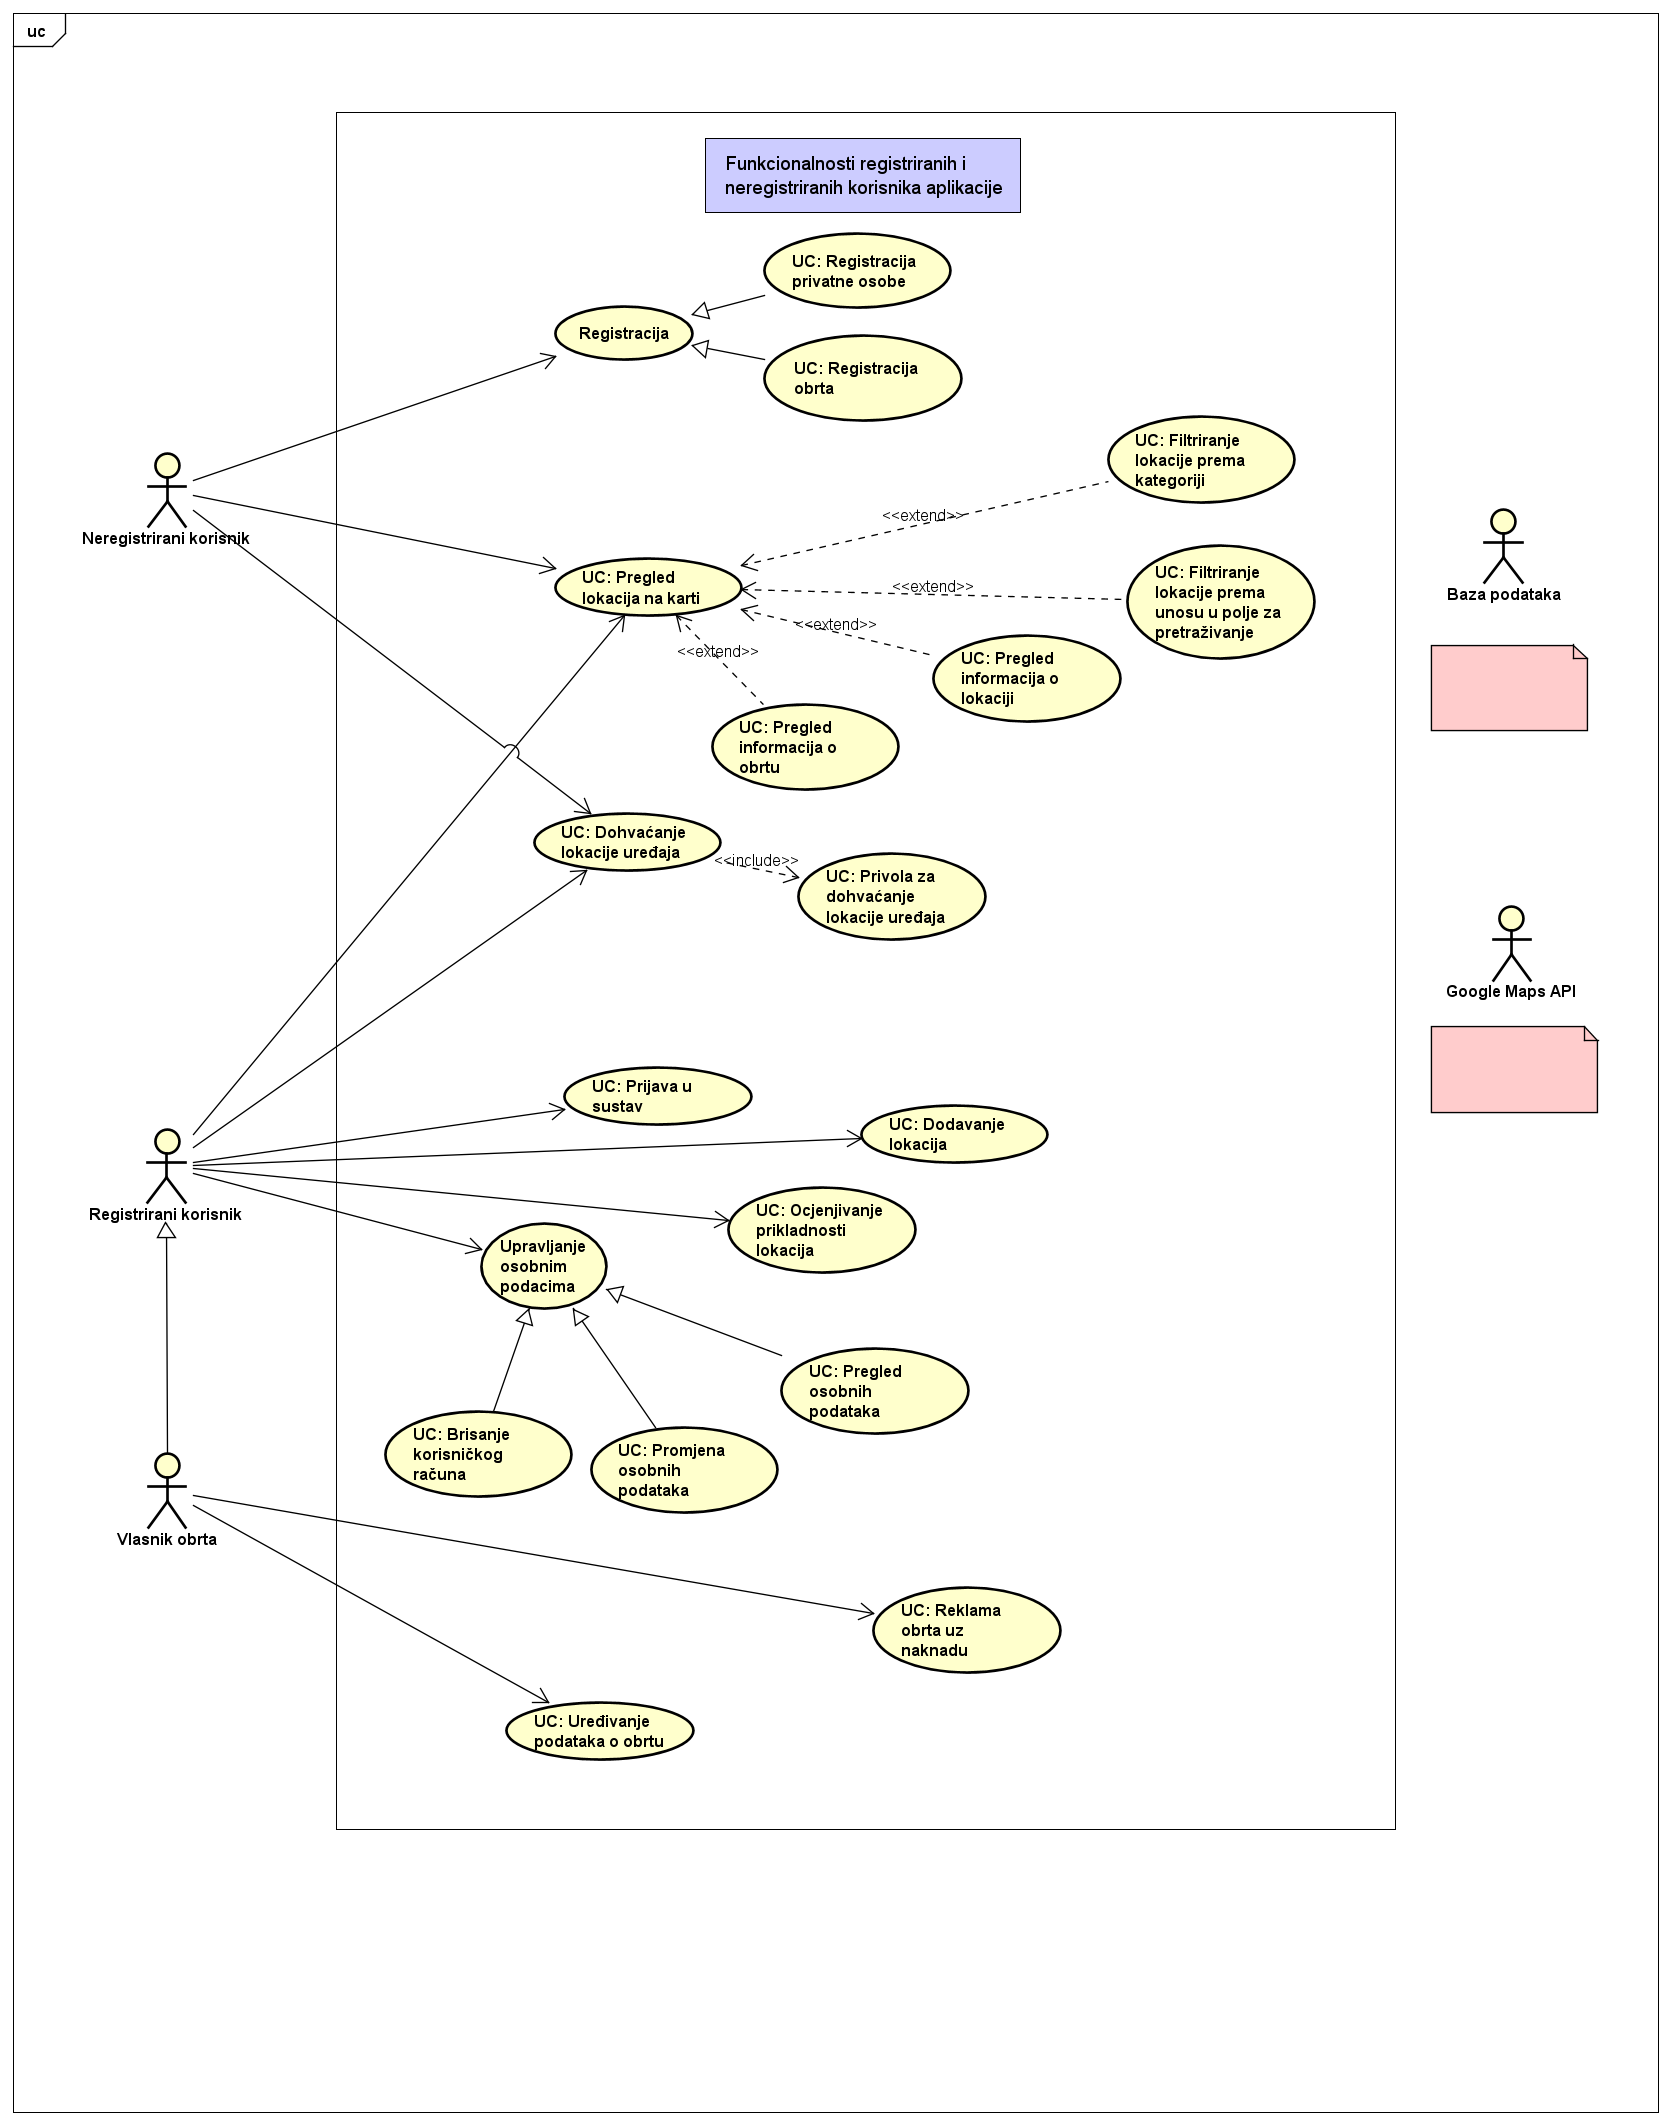
\includegraphics[scale=1.2]{slike/DijagramObrazacaUporabe1.png}
						\centering
						\caption{Dijagram obrazaca uporabe}
						\label{fig:promjene}
					\end{figure}
				\eject		
				
			\subsection{Sekvencijski dijagrami}
				
				\textbf{\textit{dio 1. revizije}}\\
				
				\textit{Nacrtati sekvencijske dijagrame koji modeliraju najvažnije dijelove sustava (max. 4 dijagrama). Ukoliko postoji nedoumica oko odabira, razjasniti s asistentom. Uz svaki dijagram napisati detaljni opis dijagrama.}
				\eject
	
		\section{Ostali zahtjevi}
		
			\textbf{\textit{dio 1. revizije}}\\
		 
			 \textit{Nefunkcionalni zahtjevi i zahtjevi domene primjene dopunjuju funkcionalne zahtjeve. Oni opisuju \textbf{kako se sustav treba ponašati} i koja \textbf{ograničenja} treba poštivati (performanse, korisničko iskustvo, pouzdanost, standardi kvalitete, sigurnost...). Primjeri takvih zahtjeva u Vašem projektu mogu biti: podržani jezici korisničkog sučelja, vrijeme odziva, najveći mogući podržani broj korisnika, podržane web/mobilne platforme, razina zaštite (protokoli komunikacije, kriptiranje...)... Svaki takav zahtjev potrebno je navesti u jednoj ili dvije rečenice.}
			 
			 
			 
	